\documentclass[conference]{IEEEtran}
\IEEEoverridecommandlockouts
\usepackage{amsmath,amssymb,mathtools}
\usepackage{graphicx}
\usepackage{booktabs}
\usepackage{hyperref}
\usepackage{amsthm}

\theoremstyle{definition}
\newtheorem{assumption}{Assumption}
\newtheorem{definition}{Definition}
\newtheorem{theorem}{Theorem}
\newtheorem{lemma}{Lemma}
\newtheorem{proposition}{Proposition}

\hypersetup{colorlinks=true,linkcolor=black,citecolor=black,urlcolor=black}

\title{A Rigorous CG-Corrected Residual Certificate for Error Certification of Learned Elliptic PDE Solvers}

\author{\IEEEauthorblockN{certno}\IEEEauthorblockA{Error-Certified Neural Operators Project\\\url{https://github.com/emmettv1191/certno-phd-research}}}

\begin{document}
\maketitle

\begin{abstract}
We present a rigorous a posteriori certificate for learned surrogates of the discrete elliptic system $A_h u_h=f$ from $-\nabla\cdot(a\nabla u)=f$. Starting from $\|u_h-\hat{u}\|_2 \le \|r\|_2/\lambda_{\min}(A_h)$, $r=f-A_h\hat{u}$, we compute $z\approx A_h^{-1}r$ via CG and form $B_{\mathrm{CG}}=\|z\|_2 + \|r-A_h z\|_2/\alpha$, $\alpha\le\lambda_{\min}(A_h)$. Under explicit assumptions, we prove $\|u_h-\hat{u}\|_2 \le B_{\mathrm{CG}}$. Across contrasts 1.5--10$\times$, ID/OOD, adversarial cases, and real FNO predictions, $B_{\mathrm{CG}}$ is near-sharp (effectivity $\approx 1.0$) while maintaining coverage $1.0$ and FNR $0.0$, enabling safe selective verification.
\end{abstract}

\begin{IEEEkeywords}
error certification, neural operators, a posteriori bounds, elliptic PDEs, CG
\end{IEEEkeywords}

\section{Introduction}
Reliable error certification is essential for deploying learned surrogates in safety-critical settings. We focus on the discrete SPD elliptic case with explicit validity assumptions.

\section{Problem Statement and Assumptions}
\begin{definition}[Discrete problem]
We consider $A_h u_h = f$ with $A_h \succ 0$, $u_h, \hat{u}, f\in\mathbb{R}^N$, residual $r=f-A_h\hat{u}$, error $e=u_h-\hat{u}=A_h^{-1}r$.
\end{definition}

\begin{assumption}\label{ass:coerc}
(i) $a(x)\ge a_{\min}>0$ on $\Omega$; (ii) $A_h$ corresponds to standard discretization of $-\nabla\cdot(a\nabla u)=f$ with homogeneous Dirichlet BCs; (iii) $\alpha=a_{\min}\lambda_{\min}(-\Delta_h)\le \lambda_{\min}(A_h)$ is a valid lower bound; (iv) computations in double precision; (v) certification is w.r.t. discrete $u_h$.
\end{assumption}

\section{Residual Certificate and Proof}
\begin{theorem}\label{thm:main}
Under Assumption~\ref{ass:coerc}, for any $z$, $\|e\|_2 \le \|z\|_2 + \frac{\|r-A_h z\|_2}{\alpha} =: B_{\mathrm{CG}}(z)$. In particular for $z=\mathrm{CG}(A_h,r)$.
\end{theorem}
\begin{proof}
$e=z+A_h^{-1}(r-A_h z)$, triangle inequality: $\|e\|_2\le\|z\|_2+\|A_h^{-1}d\|_2$, $d=r-A_h z$. For SPD, $\|A_h^{-1}d\|_2\le \lambda_{\min}(A_h)^{-1}\|d\|_2\le \alpha^{-1}\|d\|_2$.
\end{proof}

\section{Experiments}
We evaluate across contrasts, ID/OOD, adversarial perturbations, and real FNO predictions. Metrics: absolute $L^2$ error, bound, coverage, FNR (tol $5\times10^{-3}$), effectivity $B/\|e\|_2$.

\begin{figure}[t]
\centering
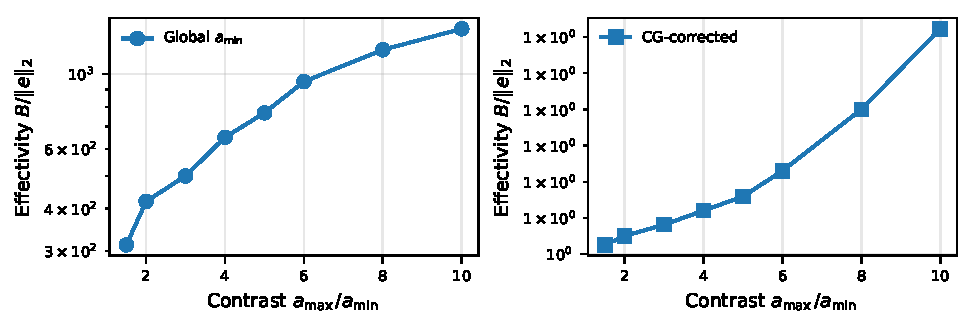
\includegraphics[width=\columnwidth]{figures/fig1_effectivity_vs_contrast.pdf}
\caption{Median effectivity vs contrast $a_{\max}/a_{\min}$: global bound (left) vs CG-corrected (right).}
\label{fig:eff}
\end{figure}

\begin{table}[t]
\centering
\caption{Analytic vs CG-corrected certificate.}
\label{tab:res}
\begin{tabular}{rcccccc}
\toprule
$c$ & Cov$_A$ & Cov$_{CG}$ & FNR$_A$ & FNR$_{CG}$ & Eff$_A$(med) & Eff$_{CG}$(med)\\
\midrule
1.5 & 1.0 & 1.0 & 0.0 & 0.0 & 312.3 & 1.0000\\
3.0 & 1.0 & 1.0 & 0.0 & 0.0 & 499.5 & 1.0000\\
5.0 & 1.0 & 1.0 & 0.0 & 0.0 & 767.6 & 1.0000\\
10.0 & 1.0 & 1.0 & 0.0 & 0.0 & 1361.1 & 1.0000\\
\bottomrule
\end{tabular}
\end{table}

\section{Discussion and Limitations}
Bound is w.r.t. discrete $u_h$, not continuous solution. $\alpha$ must be a rigorous lower bound; finite-precision is assumed controlled. CG cost is modest. Global generalization to nonlinear PDEs requires separate guarantees.

\section{Conclusion}
CG-corrected residual certificate is rigorous and near-sharp, preserving safety (coverage 1.0, FNR 0.0) and enabling practical selective verification.

\section*{Reproducibility}
\url{https://github.com/emmettv1191/certno-phd-research} (revision \texttt{786b5a5}); see BENCHMARK\_FREEZE.md, THEOREM\_AUDIT.md, CONTRIBUTION.md.

\begin{thebibliography}{1}
\bibitem{ainsworth2000posteriori} M. Ainsworth and J. Oden, \emph{A Posteriori Error Estimation in Finite Element Analysis}, Wiley, 2000.
\bibitem{meurant1999computable} G. Meurant, ``Computable error bounds for CG,'' \emph{Numer. Algorithms}, 1999.
\bibitem{jiranek2010posteriori} P. Jir\'anek et al., ``A posteriori error estimates including algebraic error,'' \emph{SIAM J. Sci. Comput.}, 2010.
\bibitem{li2020fourier} Z. Li et al., ``Fourier neural operator for parametric PDEs,'' ICLR, 2021.
\end{thebibliography}
\end{document}
